
\documentclass{beamer}
\usetheme{metropolis}           % Use metropolis theme
\title{Heavy lake-effect snowfall events for the Laurentian Great Lakes region for current and future climates}
\date{July 2019}
\author{O. Huziy\textsuperscript{1,2,3} and L. Sushama\textsuperscript{2}, L. Leon\textsuperscript{3}, R. Yerubandi\textsuperscript{3}}
\institute{
  \textsuperscript{1}Environement and Climate Change Canada,\\
  \textsuperscript{2}McGill University,\\
  \textsuperscript{3}Université du Québec à Montréal
}

\graphicspath{{figures/}}
\usepackage[export]{adjustbox}
\usepackage{array}
\newcommand{\logovspace}{0.5cm}
\usepackage{natbib}[plain]
\renewcommand*{\bibfont}{\footnotesize}

\renewcommand\bibname{}
\renewcommand\refname{}
\usepackage{tikz}
\usetikzlibrary{calc}
\usetikzlibrary{positioning}

\usepackage{xcolor}
\usepackage{bm}

% do not create a section for references
\renewcommand{\bibsection}{}

\begin{document}
  \maketitle

  \begin{frame}{Outline}
    \begin{itemize}
      \item Previous work and motivation
      \item Methods
      \begin{itemize}
        \item Models and simulation configurations
        \item Identifying HLES
      \end{itemize}

      \item Results
      \begin{itemize}
        \item HLES in current climate, validation
        \item Projected changes to HLES
      \end{itemize}
    \end{itemize}
  \end{frame}

  \section{Previous work and motivation}

  \begin{frame}{What is Heavy Lake Effect Snowfall (HLES)?}
    \centering

    \begin{columns}
      \column{0.6\textwidth}
        \begin{itemize}
            \item Lake enhanced snowfall with rates~$\geq$ 10 cm/day
            \item Required conditions:
              \begin{itemize}
                \footnotesize
                \item Unfrozen lake surface
                \item Cold air flow over lake
                \item Convergence downwind of lakes
              \end{itemize}
        \end{itemize}
      \column{0.4\textwidth}
        \centering
        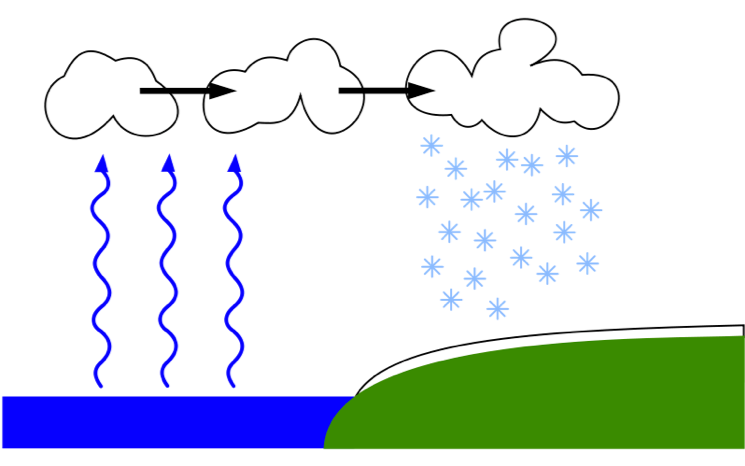
\includegraphics[width=\textwidth]{hles_sketch}
    \end{columns}

    \vspace{2em}

    \begin{columns}
      \centering
      \column{0.3\textwidth}
        \centering
        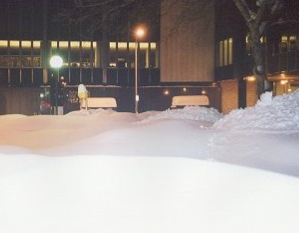
\includegraphics[height=6.5em,frame=0.05em]{hles_photo1}

      \column{0.3\textwidth}
        \centering
        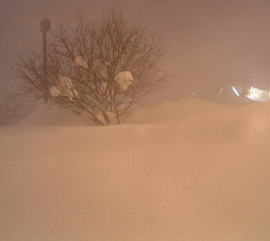
\includegraphics[height=6.5em,frame=0.05em]{hles_photo2}

      \column{0.39\textwidth}
        \centering
        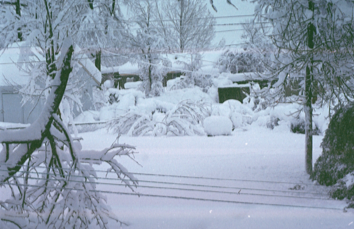
\includegraphics[height=6.5em,frame=0.05em]{hles_photo3}
    \end{columns}

  \end{frame}

  \begin{frame}{Projected changes to the number of HLES days\\ by~\citet{Notaro:2015}}
    \begin{columns}
      \column{0.6\textwidth}
        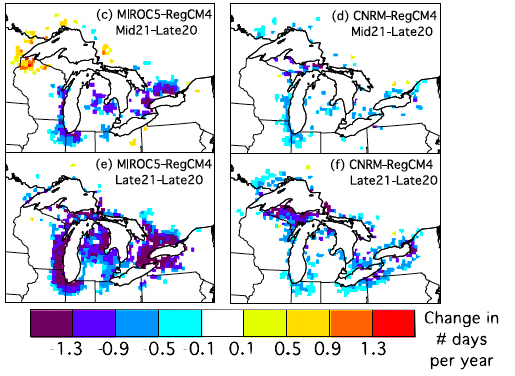
\includegraphics[height=0.6\textheight]{notaro_et_al_changes_to_hles_days.png}
      \column{0.4\textwidth}
        \begin{itemize}
          \item 1D Lake model (Hostetler)
          \item 25 km grid spacing
          \item Projected mostly decreases in the number of HLES days by the end of the 21st century
        \end{itemize}

    \end{columns}
  \end{frame}

  \begin{frame}{Objectives}
    \begin{itemize}
      \item Apply a more advanced tool to study projected changes to HLES in the Great Lakes region: coupled GEM(atm)-NEMO(lake) system.
      \item Look into how HLES is going to change during different sub-seasons of the cold season: ND, JF, MA.
      \item Study links between HLES and other near-surface and surface fields: temperature, precipitation, ice concentration in current and future climate.
    \end{itemize}
  \end{frame}

  \section{Methods}
  \begin{frame}{Models and simulation configurations}
    \begin{columns}

      \column{0.5\textwidth}
          \vspace{0.5cm}
          \includegraphics[width=\textwidth]{{sim_domain_and_focus_region}.png}
          %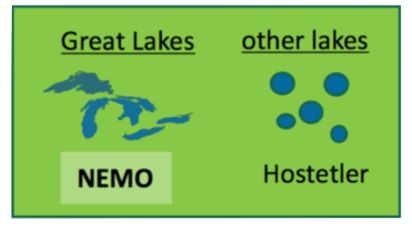
\includegraphics[width=\textwidth]{lake_parameterization_schematic.png}

      \column{0.55\textwidth}
      \begin{itemize}
        \item Horizontal grid: 452$\times$260, \textbf{0.1$^\circ$};
        \item $\Delta t$: 5 min (\textbf{GEM}), 30 min (\textbf{NEMO});
        \item Subgrid lakes: 1D lake model \textbf{Hostetler};
        \item Great Lakes: \textbf{NEMO} model with \textbf{LIM3} for lake ice;
        \end{itemize}
    \end{columns}
    \vspace{0.5cm}
    \centering

    \begin{tabular}{lll}
      \multicolumn{3}{c}{List of simulations} \\
      \hline
      \textbf{ID} & \textbf{LBC} & \textbf{Period} \\
      \hline
      GEM\_NEMO   & ERA-Interim (0.75$^\circ$) & 1980-2010 \\
      GEM\_NEMOc  & CanESM2 & 1989-2010 \\
      GEM\_NEMOf  & CanESM2 (RCP8.5) & 2079-2100
    \end{tabular}

  \end{frame}

  \begin{frame}{Identifying HLES}
    Criteria implemented based on \citet{Notaro:2015}
    \begin{columns}
      \column{0.4\textwidth}
        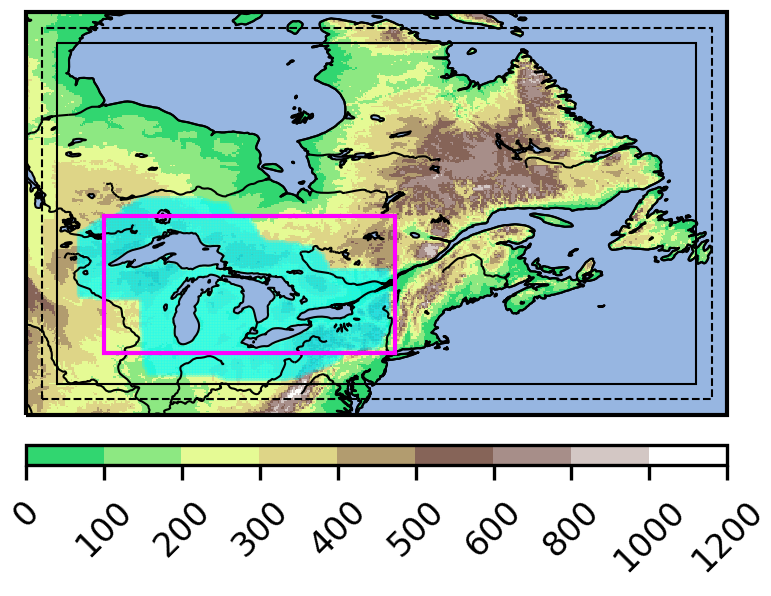
\includegraphics[width=\textwidth, trim=3cm 8cm 12.5cm 7cm, clip]{sim_domain_and_focus_region}
      \column{0.6\textwidth}
        \begin{itemize}
          \item Location within 100 km of lake shorelines
          \item 10 cm/day minimum threshold
          \item Local amplification wrt. the surrounding 500km
          \item Account for the wind fetch ($\geq$ 6 hours) from lake cells with ice cover less than 70\%
        \end{itemize}
    \end{columns}
  \end{frame}


  \section{HLES in current climate}
  \begin{frame}{Validation: spatial extent}

      \begin{figure}
        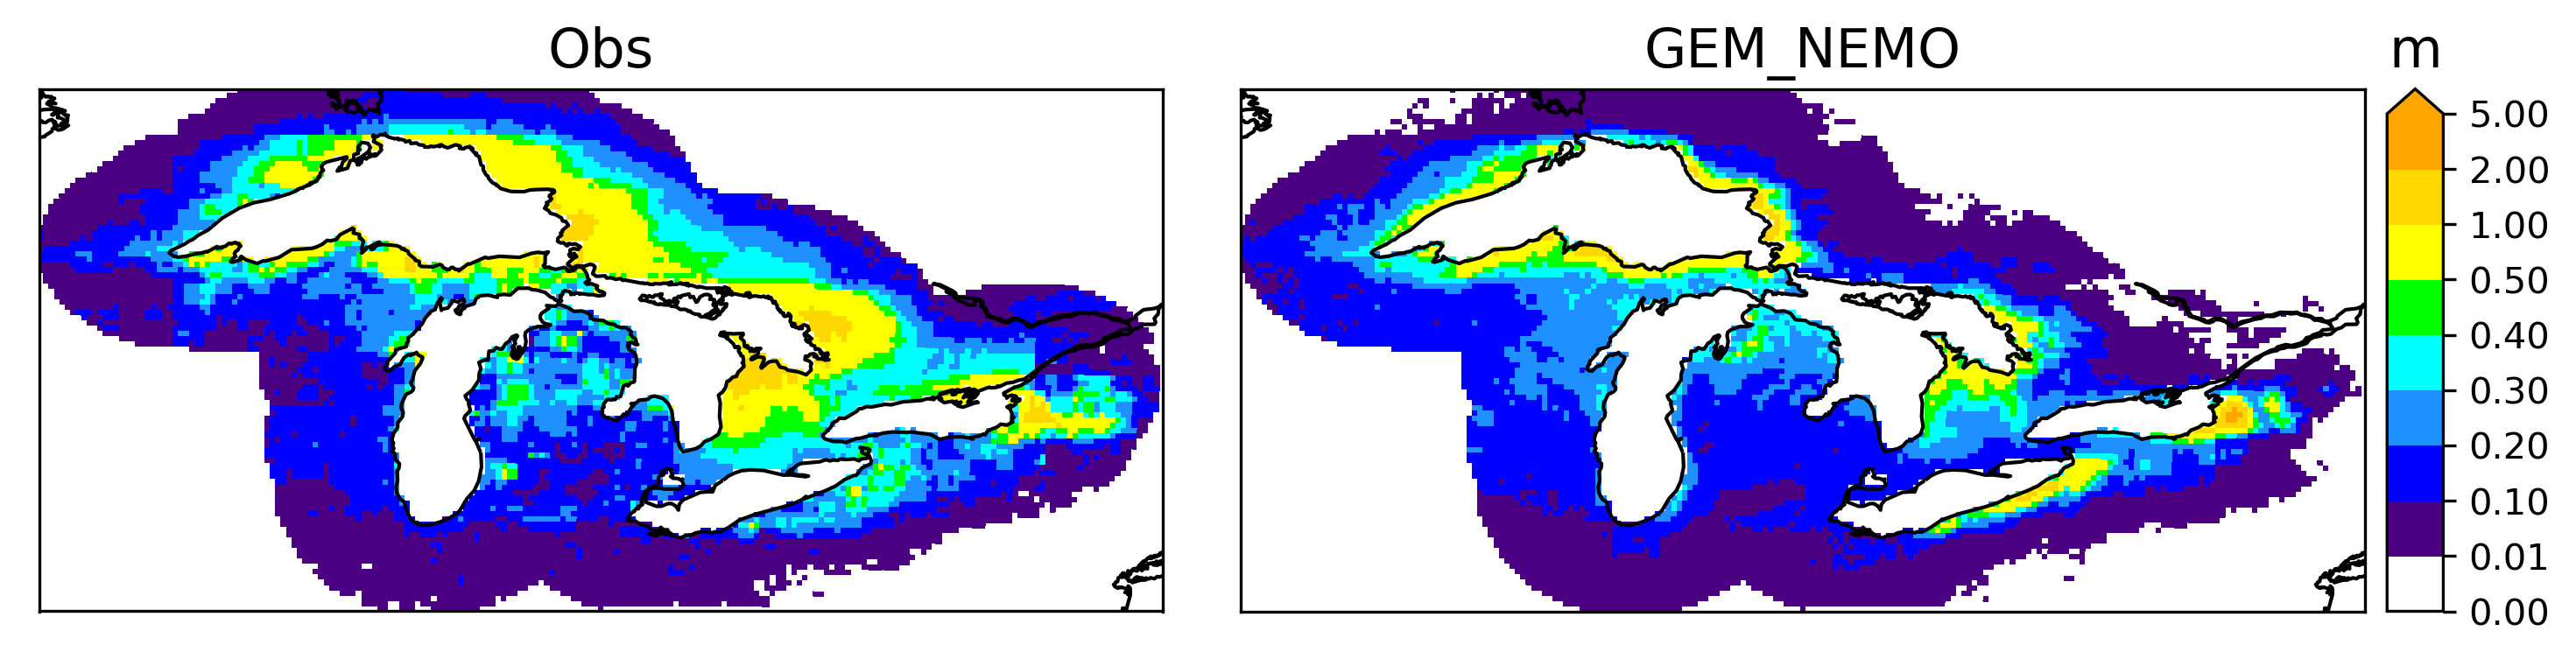
\includegraphics[width=0.9\textwidth]{hles_clim_snow_fall_1980-2009.png}
        \caption{\footnotesize Climatological (1980-2010) yearly HLES (m)}
      \end{figure}

      \begin{itemize}
        \item Observed HLES is derived from gridded observations of temperature, ice concentrations and ERA-Interim (0.75$^\circ$) surface winds
        \item Extent of HLES is mostly underestimated
        \item Overestimation downwind of lake Erie
        \item Well simulated HLES band extent downwind of lake Ontario
      \end{itemize}
  \end{frame}

  % monthly distribution
  \begin{frame}{Validation: HLES timing}

    \begin{columns}
      \column{0.5\textwidth}
        \begin{figure}
          \includegraphics[height=0.5\textheight]{{hles_histo_all_m9_10_11_12_1_2_3_4_5}.png}
          \caption{\footnotesize Monthly distribution of area-average HLES for the 1980-2010 period}
        \end{figure}

      \column{0.5\textwidth}
        \begin{itemize}
          \item Very good agreement between the model and observations during Nov and Mar
          \item Significant underestimation during Dec and Jan months, probably caused by warm temperature bias
        \end{itemize}


    \end{columns}
  \end{frame}

  \section{Projected changes to HLES}
  \begin{frame}{Projected changes to the fields impacting HLES}
    \begin{tikzpicture}[indicator/.style={scale=0.8, circle,draw=gray!60, minimum size=3.5em}]
        \node (plot) {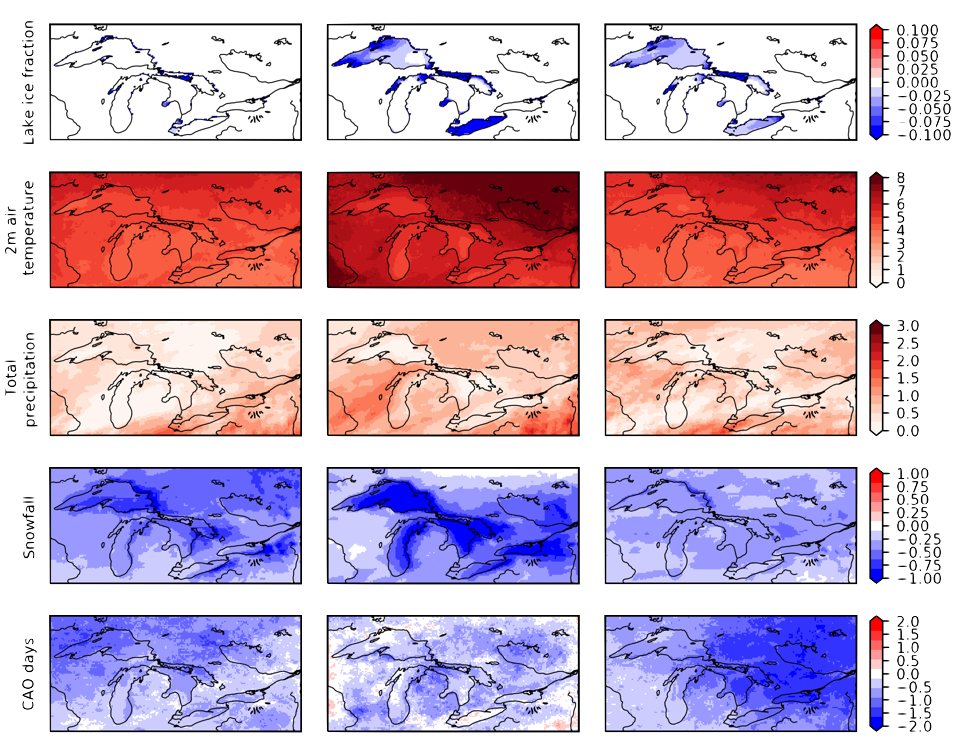
\includegraphics[height=0.85\textheight]{projected_changes_to_surf_and_nearsurf_fields.png}};
        \node[indicator, below right = 1.5em and 0.1em of plot.north east] (icesymbol) {\color{red}{$\pmb+$}\color{black}{/}\color{red}{$\pmb+$}};
        \node[indicator, below = 0.8em of icesymbol] (t2msymbol) {\color{blue}{$\pmb-$}\color{black}{/}\color{red}{$\pmb+$}};
        \node[indicator, below = 0.8em of t2msymbol] (prsymbol) {\color{red}{$\pmb+$}};
        \node[indicator, below = 0.8em of prsymbol] (snsymbol) {\color{blue}{$\pmb-$}};
        \node[indicator, below = 0.8em of snsymbol] (caosymbol) {\color{blue}{$\pmb-$}};
        %\node[below=0of plot.south]{};
    \end{tikzpicture}
    {\footnotesize {\color{red}{$+$}}/{\color{blue}{$-$}} indicate impact of changes to a field on changes to HLES.}
  \end{frame}


  \begin{frame}{Projected changes to HLES: magnitudes and frequencies}
    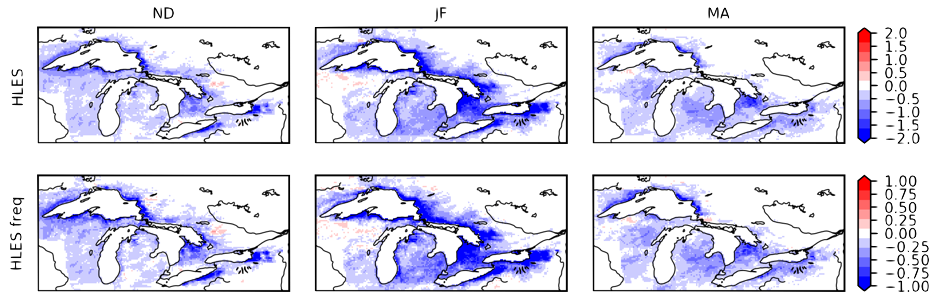
\includegraphics[width=\textwidth]{projected_changes_to_hles.png}
    \begin{itemize}
      \item Mostly decreases up to 2 cm/day
      \item Slight increases south of Lake Superior during JF and northeast of lake Huron during ND could be explained by the increased impact of lakes on the dynamics of the atmosphere
    \end{itemize}
  \end{frame}


  \begin{frame}{Area average HLES: monthly distribution\\for 1989-2010 and 2079-2100}
    \centering
    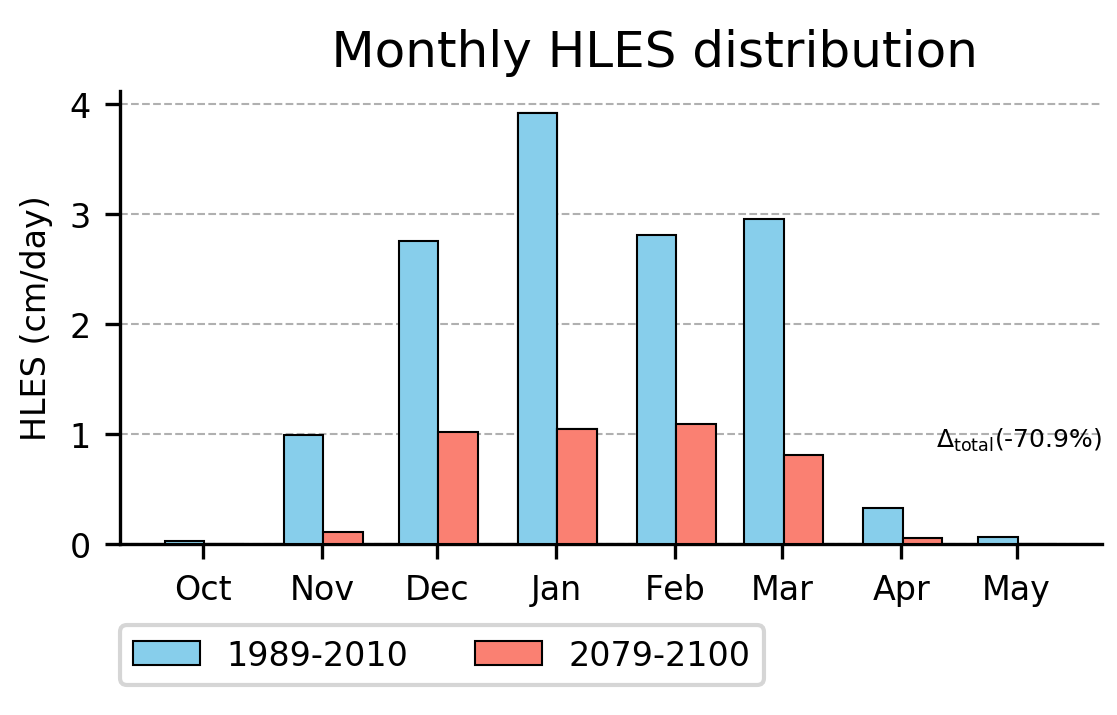
\includegraphics[height=0.55\textheight]{hles_snow_histo_cc_m10_11_12_1_2_3_4_5_domain}
    \begin{itemize}
      \item Average HLES in the domain is projected to decrease for all months
      \item HLES is projected to decrease 4 times during Jan
      \item HLES season is projected to shorten by $\approx$ 2 months
    \end{itemize}
  \end{frame}



  \begin{frame}{Mechanisms: 2m air temperature and HLES}
    \begin{tikzpicture}
      \node(plot) at (0, 0) {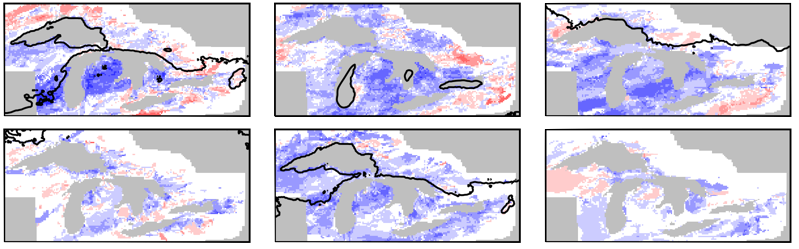
\includegraphics[width=0.9\textwidth]{t2m_vs_HLES.png}};
      \node[right=-0.5em of plot.east]{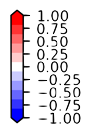
\includegraphics[width=0.12\textwidth]{corr_colorbar.png}};

      \node[above left= 0.01em and 0.01em of plot.west]{\rotatebox{90}{\footnotesize 1989-2010}};
      \node[below left= 0.01em and 0.01em of plot.west]{\rotatebox{90}{\footnotesize 2079-2100}};

      \node[above right= 0.01em and 3.2em of plot.north west] (nd) {ND};
      \node[right= 6.4em of nd] (jf) {JF};
      \node[right= 6.4em of jf] (ma) {MA};

      \node[below= 0em of plot.south]{Time correlation: 2m air temperature and HLES};
    \end{tikzpicture}

    \begin{itemize}
      \item Much weaker correlation between temperature and HLES during shoulder periods in the future
      \item Mostly negative correlation: snow to rain ratio
    \end{itemize}
  \end{frame}


  \begin{frame}{Mechanisms: lake ice concentration and HLES}
    \begin{tikzpicture}
      \node(plot) at (0, 0) {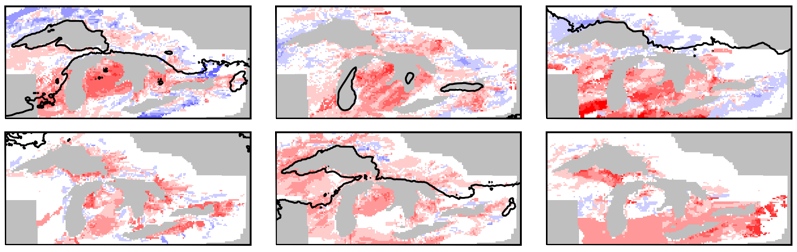
\includegraphics[width=0.9\textwidth]{lkice_vs_HLES.png}};
      \node[right=-0.5em of plot.east]{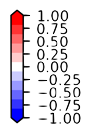
\includegraphics[width=0.12\textwidth]{corr_colorbar.png}};

      \node[above left= 0.01em and 0.01em of plot.west]{\rotatebox{90}{\footnotesize 1989-2010}};
      \node[below left= 0.01em and 0.01em of plot.west]{\rotatebox{90}{\footnotesize 2079-2100}};

      \node[above right= 0.01em and 3.2em of plot.north west] (nd) {ND};
      \node[right= 6.4em of nd] (jf) {JF};
      \node[right= 6.4em of jf] (ma) {MA};

      \node[below= 0em of plot.south](figlabel){Time correlation: lake ice concentration and HLES};
    \end{tikzpicture}

    \begin{itemize}
      \item Mostly positive correlation in the future climate: HLES decreases along with lake ice
      \item Control of ice on HLES (negative correlation) is stronger during shoulder periods (ND,MA) in the current climate
    \end{itemize}

  \end{frame}



%% No section here
  \begin{frame}{Conclusions}
    \begin{itemize}
      \item The system shows significant skill in modelling HLES even given resolution limitations.
      \item On average the HLES is projected to be less frequent and of lower intensity in the region.
      \item Slight increase in HLES magnitudes and frequencies is obtained south of Lake Superior and northeast of Lake Huron during JF and ND months respectively.
      \item Control of ice on the HLES variability is much weaker in the future period.
    \end{itemize}
  \end{frame}



  \begin{frame}{References}
    \nocite{*}
    \bibliographystyle{apa}
    \bibliography{references}
  \end{frame}


  \begin{frame}{Acknowledgements}
      \centering
      \Large{Thanks to} \\[\logovspace]
      \small
      \begin{tabular} {m{14em} l}
        \includegraphics[height=1cm]{{nserc_logo}.png} & funding \\[\logovspace]
        \includegraphics[width=10em]{{computecanada_logo}.png}  & computing and storage \\[\logovspace]
        \includegraphics[width=5.5em]{{mcgill_logo}.png} \includegraphics[width=4.5em]{{logo_uqam}.png} & base universities   \\[\logovspace]
        \includegraphics[width=14em]{{eccc_logo}.png} & models, libraries and tools \\[\logovspace]
        M. Valin, K. Winger, B. Dugas, F. Dupont and other colleagues & for their help with the project
      \end{tabular}
  \end{frame}


  \begin{frame}[standout]
    Questions?
  \end{frame}


  \begin{frame}{Mechanisms: total precipitation and HLES}
    \begin{tikzpicture}
      \node(plot) at (0, 0) {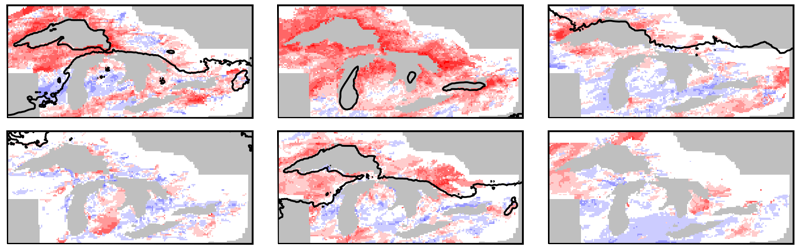
\includegraphics[width=0.9\textwidth]{pr_vs_HLES.png}};
      \node[right=-0.5em of plot.east]{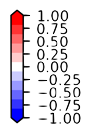
\includegraphics[width=0.12\textwidth]{corr_colorbar.png}};

      \node[above left= 0.01em and 0.01em of plot.west]{\rotatebox{90}{\footnotesize 1989-2010}};
      \node[below left= 0.01em and 0.01em of plot.west]{\rotatebox{90}{\footnotesize 2079-2100}};

      \node[above right= 0.01em and 3.2em of plot.north west] (nd) {ND};
      \node[right= 6.4em of nd] (jf) {JF};
      \node[right= 6.4em of jf] (ma) {MA};

      \node[below= 0em of plot.south]{Time correlation: total precipitation and HLES};
    \end{tikzpicture}
  \end{frame}


\appendix





\end{document}
